\documentclass[a4paper]{report}

\usepackage[margin=3.5cm,top=2.8cm,bottom=2.8cm]{geometry} %,top=0.5cm,bottom=1.8cm]{geometry}
\usepackage[svgnames]{xcolor}
\usepackage[pdftex]{hyperref}
\usepackage{amsmath,amsfonts,amssymb,amsthm,mathtools,thmtools,thm-restate,cleveref}
\usepackage{mathrsfs}   % for \mathscr "script"
\usepackage{bookmark,graphicx,dsfont,datetime,float,booktabs,multirow,siunitx}
\usepackage{enumitem,outlines,nicematrix}
\usepackage{algorithm,algpseudocode}
\usepackage{tabularx,ragged2e,adjustbox} % for literature table
\usepackage{tocloft}    % customize toc entries
\usepackage{xpatch}     % for bookmark 'hack' for appendix naming
\usepackage{setspace}   % for bookmark fix of bibliography
\usepackage{mdframed}   % for "emphasis boxes"
\usepackage{todonotes}
\usepackage{xstring}
\setlength{\marginparwidth}{3cm} % more room in margin

\usepackage{etoolbox}
% chapters in todolist
\makeatletter
\newif\ifinappendix        % define a boolean
\pretocmd{\appendix}{\inappendixtrue}{}{}  % turn on flag when appendix begins
\pretocmd{\@chapter}{%
  % Only add to list if this is a numbered chapter (not starred)
  \ifnum\c@secnumdepth>0
    \ifinappendix\else
    \addcontentsline{tdo}{todo}{\protect\textbf{Chapter \thechapter: \space}}%
    \fi
  \fi
}{}{}
\makeatother

% my custom comment command
\newcounter{mycomment}
\newcommand{\comment}[2][]{%
    \refstepcounter{mycomment}% up counter
    {%
        \setstretch{0.7}% spacing
        \StrLeft{#2}{60}[\shortcaption]% truncate text for caption
        \todo[%
        color={red!100!green!33},%
        size=\small,%
        caption={\protect\hypertarget{todo\themycomment}{}\textit{\thesubsection}%
        \hspace{1.0em}{\shortcaption}~\textit{[\themycomment]}}, #1]%
        {%
        #2~\hyperlink{todo\themycomment}{\textit{[\themycomment]}}}
    }%
}


%% bibliography setup
% \usepackage[numbers]{natbib}
% \bibliographystyle{abbrvnat}
\usepackage[
    style=numeric-comp,
    natbib=true, % enables \citet, \citep
    doi=false, isbn=false, url=false,
    maxcitenames=1,  % max one author when using \citet
    % maxbibnames=99 % show all authors
    backend=biber,
]{biblatex}
\addbibresource{references.bib}
\setlength{\biblabelsep}{0.5em}  % space between number and entry
\renewcommand*{\bibfont}{\small} % optional: font size same as natbib


%% table setup
\usepackage{tabto,caption}
% \captionsetup[table]{skip=5pt}

%% for adding floating pdf comments
% \usepackage{pdfcomment}
% \newcommand{\comment}[1]{\pdfmargincomment[author=Jeroen van Riel]{#1}}


%% tikz
\usepackage{tikz}
\usetikzlibrary{arrows.meta, decorations.markings, decorations.pathreplacing,
  positioning, fit, calc, backgrounds}

% overall text appearance
\usepackage{setspace}
% \setstretch{1.15}        % Custom spacing (1.25x)
%% micro-level typesetting
\usepackage[activate={true,nocompatibility},final,
            tracking=true,kerning=true,spacing=true,
            factor=500,stretch=15,shrink=15]{microtype}

%% theorem environments
\theoremstyle{definition}
\newtheorem{eg}{Example}[chapter]
\newtheorem{define}{Definition}[chapter]
\newtheorem{assump}{Assumption}[chapter]
\theoremstyle{plain}
\newtheorem{proposition}{Proposition}[chapter]
\newtheorem{lemma}{Lemma}[chapter]
\newtheorem{corollary}{Corollary}[chapter]
\newtheorem{theorem}{Theorem}[chapter]
\newtheorem*{remark}{Remark}
\newtheorem{remarknum}{Remark}[chapter]

%% cref settings
\crefname{equation}{equation}{equations}
\newcommand{\crefrangeconjunction}{--}

%% load styling for knitr produced tables
\input{knitr_init.tex}

%% some (math) macros
\DeclareMathOperator{\interior}{int}
\DeclareMathOperator*{\argmax}{arg\,max}
\DeclareMathOperator*{\argmin}{arg\,min}
\newcommand\halfopen[2]{\ensuremath{[#1,#2)}}
\newcommand\openhalf[2]{\ensuremath{(#1,#2]}}
\newcommand*\diff{\mathop{}\!\mathrm{d}}

\newcommand\note[1]{{\color{Navy}\noindent#1}}
\newcommand\smallnote[1]{{\color{Navy}\noindent\scriptsize#1}}

\definecolor{review}{HTML}{a0a0a0}
\newcommand\review[1]{{\color{review}#1}}

\newcommand{\TUE}{TU\kern-0.12em/\kern-0.08eme }

%% title, date and author
\newdateformat{monthyeardate}{\monthname[\THEMONTH] \THEYEAR}
\author{\Large Jeroen van Riel \\[6em] {\it Combined Master's Thesis} \\[0.6em] Industrial and Applied Mathematics \\ Computer Science and Engineering  \\[3em] {\it Supervisors} \\[0.6em] Marko Boon \\ Stella Kapodistria \\ Mykola Pechenizkiy \\ Danil Provodin  \\[8em] October 2025 \\[0.6em] Eindhoven University of Technology}
\date{}
\newcommand{\mytitle}{%
  {\huge\bf Drive Safe!}\\[3.0em]
  {\Large\bf Combinatorial Optimization Problems}\\[0.0em]
  {\Large\bf in }\\[0.0em]
  {\Large\bf Autonomous Traffic Coordination}}
\title{\mytitle}

% links setup
\colorlet{redcustom}{red!80!black}
\colorlet{bluecustom}{blue!60!black}
\hypersetup{
    colorlinks=true,       % Use colored text instead of boxes
    linkcolor=redcustom,   % Color of internal links (sections, figures)
    citecolor=bluecustom,  % Color of citations
    filecolor=redcustom,   % Color of file links
    urlcolor=redcustom,    % Color of URLs
    breaklinks=true,       % Allows links to wrap across lines
    % hypertexnames=false,   % Avoids duplicate anchor names
}

%% set pdf meta-data
\hypersetup{
    pdftitle = {Drive Safe! Combinatorial Optimization Problems in Autonomous Traffic Coordination},
    pdfauthor = {Jeroen van Riel}
}

\begin{document}

\chapter{Machine learning for combinatorial optimization}\label{chap:ml-co}

\section[Context and motivation]{Context and motivation\footnote{The narrative of this section has
    been heavily influenced by the presentation
    in~\cite{bengioMachineLearningCombinatorial2020} and we have borrowed some
    of their notation to explain the algorithm optimization problem over problem
    distributions.}}

Recent years have seen increased research interest in using models and methods
from the machine learning (ML) community for solving combinatorial optimization
problems (CO).
%
In this chapter, we first discuss some key ideas and techniques found within
this line of work.
%
Based on this, the next chapter details our own version of this methodology for
solving the crossing time problem introduced in Chapter~\ref{chap:single}.

In typical CO problems, we try to find some the best option from some set of
discrete structures such as graphs, sets, sequences, etc.
%
Typical problems involve, for example, finding some path or route through a
graph, like in the traveling salesman problem; selecting some optimal subset,
like in the knapsack problem or set cover problem; or selecting the best
sequence in which machines are assigned to pending jobs, as in job-shop
scheduling.
%
Generally speaking, we can think of CO problems as being concerned with finding
an optimal configuration vector $v \in V$ from a finite\footnote{This assumption
  simplifies our current discussion, but note that some typical combinatorial
  problems have infinitely many feasible solutions.
%
  It is not trivial to distinguish between \emph{continuous} optimization
  and \emph{combinatorial} optimization.
%
  We could call a problem combinatorial if at least one component $v_i$ of the
  configuration $v \in \mathbb{R}^n$ is restricted to lie in some countable domain.
%
  For example, this is the case for mixed-integer programs, where some
  variables are restriced to the integers.
%
  However, some problems that should be called continuous according to this
  definition are more combinatorial in nature than it seems at first sight. For
  example, the feasible set of a linear program is generally not a finite set,
  but Dantzig's simplex algorithm shows that the optimal solution must be one of
  the finitely many vertices of the convex polytope.} set of candidates, such
that some objective function $f : V \rightarrow \mathbb{R}$ is minimized.
%
Since there are only finitely many candidates, a straightforward solution is to
just evaluate the objective for each candidates $v \in V$ and then output some
configuration for which $f(v)$ is minimal.
%
However, for all but trivial problems, this is simply not feasible in any
reasonable amount of time, which is the central motivation in the field of
combinatorial optimization.

In almost all practically relevant CO problems, the \emph{objective} function
$f$ exhibits some kind of regularity.
%
Therefore, when developing algorithms, a good strategy is to look for such
structure in the problem that can be exploited algorithmically.
%
% proofs -> algorithmic ideas with optimality guarantees
Such structural insights can be precise, like in Theorem~\ref{thm:exhaustive}, and methods like
those based on the branch-and-bound scheme try to take advantage of such
well-defined structure. Often, such algorithms come with some kind of guarantee
on the quality of the returned solution.
%
% intuition -> algorithmic ideas without guarantees
Other algorithms are based on some hard-to-define intuition about what optimal
solutions should look like.
%
This very much applies to so-called \emph{local search} algorithms.

\paragraph{Literature overview.}
Within this context, two main motivations for applying ML for solving CO
problems can be identified in the current
literature~\cite{bengioMachineLearningCombinatorial2020}, which we discuss next.
%
The key publications on which the following discussion is based are collected in
Table~\ref{tab:ml-co-literature}.

\emph{1. Fast approximations.}
%
We might want to replace certain expensive computations of an existing
algorithms such as branch-and-bound with fast ML approximations.
%
Please note that the approximate nature of ML models does not necessarily impact
optimality guarantees of the original algorithm.
%
This is clearly illustrated by~\cite{gasseExactCombinatorialOptimization2019}, where the branching decision in
branch-and-bound is approximated, and the line of work related to~\cite{tangReinforcementLearningInteger2020}, where
ML models are employed for cutting plane selection.
%
In both examples, the algorithm is still guaranteed to obtain an optimal
solution, as long as the model provides valid branching decisions or valid
cutting planes.
%
Schemes in which ML models are integrated within some existing CO algorithm have
been referred to as \emph{joint} methods.

\emph{2. Algorithm discovery.}
%
Instead of trying to improve existing algorithms, we could try to employ ML to
explore the space of algorithms to find new, hopefully better, algorithms.
%
This type of approaches can also be understood as constructing a solution from
scratch or in terms of predicting the optimal solution, given the problem
instance.
%
Our method, that we will propose in~\Cref{chap:single-learning}, belongs to this
class of so-called \emph{principal} methods.

\paragraph{Central ideas.}
In both cases, the premise is that \emph{ML can be used to discover certain
  regularities of the problem automatically}.
%
Therefore, one of the central ideas is to treat problem instances and their
solutions and training data for a machine learning model~\cite{bengioMachineLearningCombinatorial2020}.
%
This training data is used to fit a machine learning model and the hope is that
it somehow captures model structure similar to our intuition.
%
In the next section, we will make this notion more precise by presenting
the process of designing algorithms for CO problems as an optimization problem
in and of itself.
%
After that, we show how to state this in terms policy optimization in some
Markov decision process (MDP), opening up the application of optimization
methods from reinforcement learning.

\newcolumntype{L}[1]{>{\RaggedRight\hsize=#1\hsize\hspace{0pt}}X}
\begin{table}
\centering
\renewcommand{\arraystretch}{1.2}

\begin{adjustbox}{center}
\scalebox{0.8}{
\begin{tabularx}{1.4\textwidth}{@{} l L{0.5} L{1.5} @{}}
\toprule
\textbf{Reference} &
\textbf{Problem focus} &
\textbf{Contribution / Method} \\
\midrule
\citet{bengioMachineLearningCombinatorial2020} & General CO problems & Survey on using ML for CO, framing the learning problem \\
\citet{mazyavkinaReinforcementLearningCombinatorial2020} & General CO problems & Survey on using ML for CO, with a focus on reinforcement learning \\
\citet{daiLearningCombinatorialOptimization2018} & Graph problems & Deep RL with graph embeddings to construct solutions \\
\citet{vinyalsPointerNetworks2017a} & TSP & Pointer networks for sequence-based combinatorial problems \\
\citet{koolAttentionLearnSolve2019} & Routing problems & Attention model trained with RL for solving TSP, VRP \\
\citet{gasseExactCombinatorialOptimization2019} & MILP & Approximate strong branching policy with GNNs in branch-and-bound \\
\citet{tangReinforcementLearningInteger2020} & ILP & Attention-based model for cutting plane selection trained with RL \\
\citet{gravesNeuralTuringMachines2014} & General computation & Neural turing machine as a differentiable model of universal computation \\
\bottomrule
\end{tabularx}}
\end{adjustbox}
\caption{Some key references on machine learning for combinatorial optimization.}%
\label{tab:ml-co-literature}
\end{table}


\subsection{Optimizing the algorithm}

% The process of designing an algorithm itself may be considered as an
% optimization problem.
%
Let $\omega = (V, f) \in \mathcal{I}$ denote some particular instance of a
combinatorial problem and let $\pi \in \Pi$ denote some set of possible
algorithm for solving it---we will make the definition of $\Pi$ more precise
later.
%
Let $m : \mathcal{I} \times \Pi \rightarrow \mathbb{R}$ denote some function
that measures the performance of executing algorithm $\pi$ on problem instance
$\omega$. Function $m$ may involve aspects like whether the algorithm actually finds
a valid solution, optimality of the found solution, running time and usage of
other resources like memory, etc.
%
Using this notation, the goal of the algorithm developer can be succintly
formulated as
\begin{align}
  \min_{\pi \in \Pi} m(\omega, \pi) .
\end{align}
However, this single-instance situation is not very typical. More often we have
some class of instances $\mathcal{I}$ of interest, say, the set of all traveling
salesman problems.
%
Let $m(\omega, \pi)$ measure the running time of the algorithm, then from the
perspective of the classical worst-case running time analysis, the algorithm
developer's goal is now
\begin{align}
  \label{eq:min-max-runtime}
  \min_{\pi \in \Pi} \max_{\omega \in \mathcal{I}} m(\omega, \pi) .
\end{align}

\paragraph{Problem distribution.}

In principle, we wish to devise algorithms that perform as good as possible for
all possible instances $\mathcal{I}$. However, in most practical application, we
are only dealing with a narrow subset of $\mathcal{I}$, often consiting of very
similar problems.
%
To model the relative occurence and/or importance of problems, we can induce a
probability distribution $P$ over $\mathcal{I}$.
%
To illustrate this, imagine some delivery company in Eindhoven that needs to
solve many instances of the vehicle routing problem (VRP) every day~\cite{bengioMachineLearningCombinatorial2020}. The
problems they encounter are often similar in some sense: many customers are
located in the north, there is one large customer in the south, only a few
regular customers are located at the \TUE campus; it often turns out to be
beneficial to plan routes that use the ring road, etc. The company does not care
about solving all possible VRPs, just their particular kind. This example is
further illustrated in Figure~\ref{fig:problem-distribution}.

There is some underlying, but unknown, probability distribution $P$ describing the
instances the company will likely face.
%
This distribution captures the problem instances the company actually cares
about.
%
Hence, instead of~\eqref{eq:min-max-runtime}, the company is actually more
interested in\comment{The free lunch theorem also motivates this sharper definition.}
\begin{align}
  \label{eq:max-expected-performance}
  \min_{\pi \in \Pi} \mathbb{E}_{\omega \sim P} \left[ m(\omega, \pi) \right] .
\end{align}
%
However, since $P$ is generally inaccessible, we need to resort to using
samples, which could be obtained from historical company data, for example.
%
Suppose that we have some set of training instances $D_\text{train} \sim P$ at
our disposal, then we could approximate~\eqref{eq:max-expected-performance} by solving
\begin{align}
  \min_{\pi \in \Pi} \sum_{\omega \in D_\text{train}} \frac{1}{|D_\text{train}|} m(\omega, \pi) .
\end{align}


\begin{figure}
  \centering
  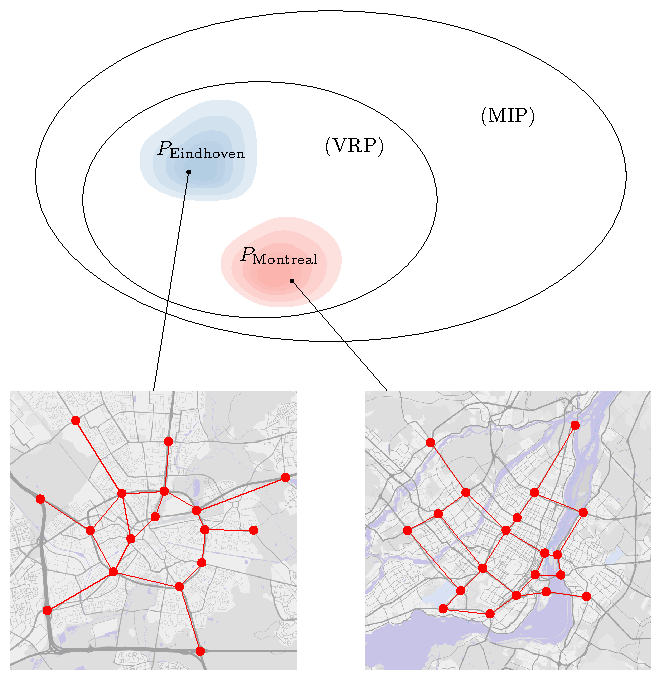
\includegraphics[scale=1]{figures/problem-distribution.pdf}
  \caption{\emph{Illustration of how problems occuring in practice have a
      naturally narrow distribution within the full space of problem.}
    %
    The top of the figure illustrates a typical hierarchical relationship between classes
    of combinatorial problems: instances of the vehicle routing problem (VRP)
    can be understood as specific instances of mixed-integer programs (MIP) and this relationship is mathematically well-defined.
    %
    In contrast to this clear boundary between problems, it might make more
    sense to consider a less sharp boundary between classes of problems by
    considering their distribution instead.
    %
    For example, we might consider the distribution $P_\mathrm{Eindhoven}$ of
    VRPs encountered by some imaginary delivery company in Eindhoven. The left graph
    illustrates what a typical sample from this distribution could look like.
    %
    Suppose that the delivery company also has an overseas branch in Montreal,
    then the distribution $P_\mathrm{Montreal}$ of
    problems faced by that branch will be very different.
    %
    For example, the Dommel river does not have such a large influence on the
    connectivity in Eindhoven compared to that of the St. Lawrence River.
    Furthermore, Eindhoven has some sort of circular connectivity due to the
    ring road, whereas large parts of Montreal are fairly Manhattan-like. It
    should be clear that statements like these are very cumbersome to formalize
    precisely, which is one of the main motivations for exploring how machine
    learning can be applied to such problem settings.}\label{fig:problem-distribution}
\end{figure}


\paragraph{Class of algorithms $\Pi$.}
To make the algorithm optimization idea outlined above more concrete, we first
need to fix a suitable representation for the set of algorithms $\Pi$. In
principle, we could take $\Pi$ to consist of all possible C programs, or all
Python programs, for example. However, real-world code runs on a complex stack
of compilers, interpreters, and other complicating factors like hardware
optimizations. Therefore, it might be more desirable to work with simplified
models of computation. A common modeling choice in the ML for CO literature is
to represent algorithms as policies for Markov decision processes (MDPs). This
perspective naturally connects algorithm optimization to reinforcement learning
methods, which many existing works indeed
leverage~\cite{mazyavkinaReinforcementLearningCombinatorial2020,daiLearningCombinatorialOptimization2018,koolAttentionLearnSolve2019}.
In what follows, we show how the MDP framework arises naturally as a model of
computation and explain why it provides a particularly useful abstraction within
the contex of algorithm optimization.

\subsection{A model of computation}

% DFA = base model
A key idea in the existing ML for CO literature is to model the class of
candidate algorithms in terms of policies for some Markov decision process
(MDP).

\paragraph{Finite-state automaton.}
First, we show how the execution of an algorithm can be viewed as a particular
state transition sequence of some deterministc finite-state automaton (DFA). Let
$\mathcal{S}$ be the finite set of states, with
$\mathcal{S}_0 \subseteq \mathcal{S}$ denoting the initial states, encoding
problem instances, and $\mathcal{S}_f \subseteq \mathcal{S}$ denoting the final
states that represent possible outputs. The remaining states capture the
\emph{internal state} of the algorithm, consisting of all relevant data
structures in memory.
%
Let $\mathcal{A}$ denote the finite non-empty set of \emph{actions}\footnote{Note that
  ``input alphabet'' is actually more common terminology for DFAs, because of
  their origins in complexity theory and formal languages, where they are
  usually defined in terms of \emph{accepting} or \emph{rejecting} a certain sequence of input
  symbols depending on the final state. In some sense, they are strictly less
  powerful than Turing machines; the latter is generally regarded as the most
  powerful/complete model of computation (Church-Turing thesis).}
%
and let $p : \mathcal{S} \times \mathcal{A} \to \mathcal{S}$ be some
\emph{transition function} that specifies the next state when a particular
action is chosen.
%
In this context, an algorithm can be viewed as a \emph{policy} function
$\pi : \mathcal{S} \rightarrow \mathcal{A}$ that provides the action to be taken
from each state.
%
The policy parameterizes the automaton’s execution similar to how program code
determines the state transitions of a computer.
%
% performance measure
In this model, the performance of running algorithm $\pi$ on instance $\omega$ is
measured\footnote{To accomodate this, states may need to carry auxiliary
  meta-information such as total number of transitions or bounds on the quality
  of the solution. Actual running time is not captured by this simple model
  formulation, but the number of transitions can be used as a proxy. This is no
  immediate problem: the current model is merely used as a way of introducing
  the general methodology.} in terms of the unique final state $s_f^\pi$ by some
cost function $c : \mathcal{S}_f \rightarrow \mathbb{R}$, such that we have
$m(\omega,\pi) = c(s_f^\pi)$.

% optimization and restriction of $\Pi$ through choice of $\mathcal{S}$
\paragraph{Designing the automaton.}

With this model in hand, we can now define $\Pi$ to be the set of valid policy
functions for some fixed automaton.
%
Hence, the automaton definition becomes a key decision in the algorithm
optimization, because fixing a particular state space effectively restricts the
class of algorithms.
%
The algorithm designer can choose to use a very general automaton, similar to a
Turing machine, or incorporate prior knowledge and intuition by carefully
defining a more restricted state space.
% example: local search
To illustrate this, suppose we let the state space represent all possible
permutations of nodes in a traveling salesman problem, then $\Pi$ would
naturally model all possible local search algorithms.
%
Indeed, any permutation of the nodes corresponds to a valid tour such that any
state is a valid solution, so we have $\mathcal{S}_f = \mathcal{S}$.
%
The transition function $p$ implicitly defines the \emph{neighborhood} of each
solution, and the policy $\pi$ specifies which neighbor to choose, capturing the
essence of the local search process.

% towards MDP
\paragraph{Markov decision process.}
We can generalize the automaton defined above as follows.
% stochastic transitions
% stochastic policy
Instead of a single next state, the transition function $p$ becomes a mapping to
distributions of states.
similarly, we let policies map to distribution over actions.
Therefore, we now write
\begin{align*}
  p : \mathcal{S} \times \mathcal{A} \rightarrow \Delta(\mathcal{S}) \quad \text{ and }
  \quad \pi : \mathcal{S} \rightarrow \Delta(\mathcal{A}) .
\end{align*}
%
This generalization turns the automaton into a finite-horizon MDP, with $r = {-c}$
taking the role of final reward function.
%
To take into account the additional stochasticity this introduces, we can generalize the algorithm development objective~\eqref{eq:max-expected-performance} to
\begin{align}\label{eq:max-mdp-performance}
  \max_{\pi \in \Pi} \mathbb{E}_{\omega \sim P} \left[ \, \mathbb{E}_\pi \left[ r(s_f^\pi) \mid \omega \right] \, \right] ,
\end{align}
where the inner expectation corresponds to the randomness of policy evaluation
in the MDP, because $s_f^\pi$ is now a random variable, and $\Pi$ still denotes
the set of all \textbf{deterministic} policies.

% stochastic transitions
\paragraph{Why is stochasticity useful?}
It might not be immediately clear why we would want to introduce stochasticiy in
a seemingly deterministic problem environment.
%
We will discuss two reasons why the MDP framework is nevertheless an attractive
starting point.

First of all, non-deterministic transitions can be used to model certain parts
of the computation that are too complex to model explicitly.
%
This has for example been done in previouw joint methods, in which some part of
an existing CO solver is augmented by replacing a specific component with a ML
model.
%
For example, we might take some existing integer programming solver as the base
algorithm, while parameterizing a specific component, say, cutting plane
selection, as done in~\cite{tangReinforcementLearningInteger2020}.
%
In that case, the actions $\mathcal{A}$ correspond to selecting some valid
cutting plane, upon which the state transition $p$ models the whole of the
execution of the solver until the next time a cutting plane has to be selected.

Although the final policy should be deterministic, during the optimization of~\eqref{eq:max-mdp-performance}, stochastic policies might be considered.
%
The reasons for this are mainly of a technical nature, for example to promote
exploration or to make sure the policy gradient exists. Alternatively, we could
interpret action probabilities as modeling the uncertainty about which actions
are optimal.
%
In some sense, this is similar to the practice of considering \emph{relaxations}
when solving integer programs. In the relaxed version of an integer program, the
integer constraints are removed, which makes it much easier to solve. Of course,
the final solution must satisfy the integer constraints, so we need some sort of
\emph{rounding procedure} to return to integer values.
%
Similarly, we eventually want to find an optimal deterministic policy, but we
relax the ``determinism constraint'' by allowing distributions of actions
instead.
%
We need to specify some ``rounding procedure'' to return to deterministic (also
called \emph{degenerate}) distributions, for example, by performing greedy
action selection, or by other search procedures proposed like \emph{active
  search}~\cite{belloNeuralCombinatorialOptimization2017} or \emph{beam
  search}~\cite{koolLearningOptimizationCombinatorial2022}.

\pagebreak[4]
\paragraph{\textit{Computing MDP} framework.}

We now summarize the algorithm optimization paradigm, outlined above, by listing
the main components of the MDP and their modeling role:

\begin{mdframed}
\begin{enumerate}[label=$\bullet$,leftmargin=2.5em,rightmargin=4em,midpenalty=5]
  \item The \textbf{state space} models all configurations of the \emph{internal state}
        of the algorithm. These may correspond to hand-crafted, problem-specific
        data structures or more model actual computer memory more generally.

  \item The set of \textbf{actions} may be thought of as the \emph{instruction set}.

  \item The \textbf{state transitions} determine how these instructions are executed.
        Stochastic state transition can be used to model fixed parts of existing
        algorithm that are too complex and expensive to consider in their
        entirety.

  \item The \textbf{reward function} measures how well an algorithm performs when
        executed on a particular problem instance.

  \item The goal is to find a \textbf{deterministic policy} that
        maximizes~\eqref{eq:max-mdp-performance}. Stochastic policies are
        considered during optimization for technical reasons.
\end{enumerate}
\end{mdframed}

% \vspace{0.5em}

% \begin{figure}
%   \centering
%   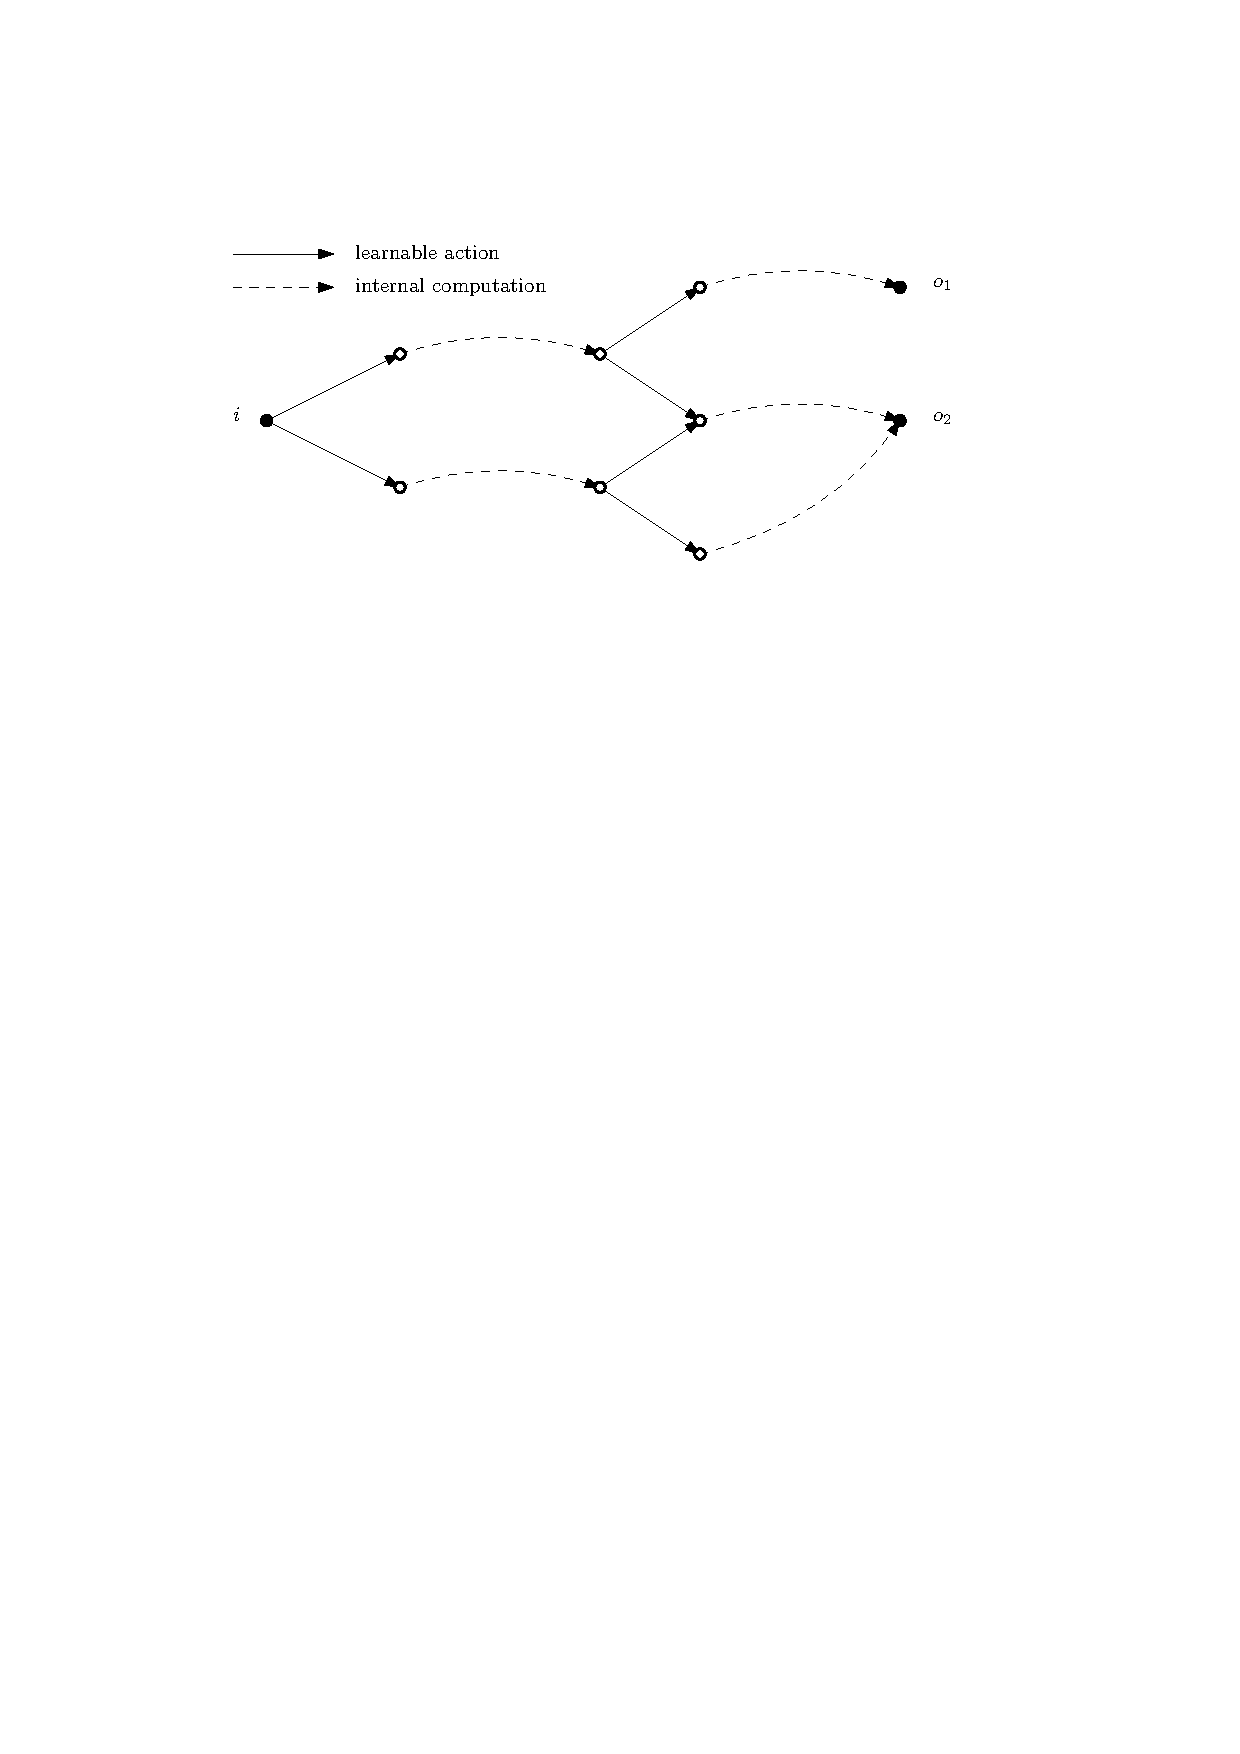
\includegraphics[scale=1]{figures/algorithm-automaton.pdf}
%   \caption{Schematic of how the computation automaton models parameterized
%     decisions in certain parts of the algorithm. Open dots represent sets of
%     internal states of the algorithm, modeled as single states in the MDP. The
%     final states $o_1$ and $o_2$ are possible output of the algorithm, encoding
%     feasible solutions.}\label{fig:algorithm-automaton}
% \end{figure}

\begin{remark}
  Within the above framework, we can also think about the analogy between
  procedures, in computer code, and the \emph{options
    framework}~\cite{suttonMDPsSemiMDPsFramework1999}, which is a classical
  approach of temporal abstraction in MDPs.
\end{remark}

\begin{remark}
  A closely related line of research that takes the above paradigm to the
  extreme is the study of \emph{Neural Turing Machines}~\cite{gravesNeuralTuringMachines2014}, where neural
  networks are used to parameterize the execution of a Turing machine, which is
  in some sense a universal and complete model of computation.
  %
  It has been demonstrated that simple algorithms for tasks such as sorting or
  information retrieval can, in principle, be ``learned from experience'' in
  this way.
  %
  While this represents a conceptually powerful idea, in
  practice such models are notoriously difficult to train. The vast space of
  possible policies effectively imposes only a very weak prior. Consequently, it
  is often more practical to design parameterizations that are better aligned
  with specific problem structures, thereby improving convergence.
%
  In this light, our own MDP formulation of~\Cref{sec:MDP}, can be understood as
  introducing a particularly strong prior.
\end{remark}

\begin{remark}
  Regarding the use of probabilities in the model, note that the transition
  probabilities in the MDP do not necessarily represent any inherent randomness
  in the system. The underlying computational process is, in principle, fully
  observable and deterministic, meaning that the exact state can always be
  known. Therefore, there is no \emph{aleatoric uncertainty} associated with the
  system. However, as discussed above, it can still be useful to represent
  certain components of the computation probabilistically. In this case, we are
  modeling \emph{epistemic uncertainty}---that is, uncertainty arising from
  incomplete knowledge or imprecise information, which could, in principle, be
  reduced by gaining more data or understanding.
\end{remark}


\clearpage
\section{Overview of methodology}

We argued that the algorithm optimization problem sketched above can be
naturally stated in terms of finding an optimal policy in some MDP.
%
This enables us to draw from the vast reinforcement learning literature for
policy optimization methods.
%
We outline a general methodology, centered around the follow three
aspects.
%
First, we explain that (i) generalization should be regarded a key objective.
%
Obtaining policies that generalize well also justify the typically long time
needed for traning, which can happen offline.
%
Next, we discuss two important engineering-type aspects, which are (ii) the way
in which the policy is parameterized and (iii) the corresponding optimization
procedure.

\paragraph{Performance evaluation.}

\note{Performance evaluation is mainly based on expected solution quality and on
  expected running time. Return to the issue of measuring running time using the
  MDP model.}

\subsection{Generalization}

One of the main challenges in ML for CO is obtaining algorithms that generalize
to instances not seen during training.
%
This means that the learned policy should not only perform well on the training
data set but also remain robust when facing instances from $P$ not seen before
in $D_\text{train}$.
%
For this reason, it makes sense to use a set of validation samples
$D_\text{valid}$ to gauge how well the learned policy generalizes to unseen
instances.

Because we are dealing with sequential decision making models, we emphasize that
generalization also applies to \emph{unseen internal states}.
%
We want policies that do not break down immediately when slightly different
internal states are encountered---for example, when some decision early on leads
to a novel configuration of the remaining algorithmic state that was rarely, if
ever, observed during training.
%
It has been observed that policy optimization with RL techniques, compared those
based on the imitation learning principle, which we will discuss in more detail
below, can help improve
generalization~\cite{belloNeuralCombinatorialOptimization2017}. This is not
surprising, since RL methods are specifically designed to explore the state
space actively.
%
Unlike imitation learning, which is constrained by the trajectories of an
expert, RL encourages the discovery of alternative strategies and adaptation to
unseen states, which tends to foster robustness.

There are two important axes to consider when measuring generalization
capabilities: instance \emph{size} and instance \emph{structure}.
%
For example, in the traveling salesman problem (TSP), the number of nodes is a
natural measure of size: scaling from 20 nodes to 100 nodes dramatically
increases the size of the solution space. A well-generalizing policy should
gracefully adapt to scaling up or down, even if it has only been trained on a
narrow size range.
%
The \emph{structure} axis, on the other hand, refers to the occurence of patterns or
lack of them within problem instances. For TSP, this might include differences
between uniformly random point clouds, clustered distributions of nodes, or
instances derived from real-world city layouts. Policies that generalize well
with respect to structural differences should be able to transfer knowledge
about synthetic training data to instances encountered in the real-world.

In practice, strong generalization requires balancing both axes: a policy that
scales to larger sizes but fails to adapt to structural changes is just as
limited as one that can handle different structures but collapses under size
increases.


\subsection{Policy parameterization}

\note{Why parameterize at all? Because it is not guaranteed that the policy space is finite.}
% why parameterize? vs. "tabular methods"
In the context of CO problems, we can safely assume that the state and action
space are discrete (countable).
%
In principle, the deterministic policy $\pi : \mathcal{S} \rightarrow \mathcal{A}$ or
stochastic policy $\pi : \mathcal{S} \rightarrow \Delta(\mathcal{A})$ can thus be represented by
a look-up table, mapping each state to an action or action distribution,
respectively.
%
However, such a tabular method becomes intractable very quickly, because the
size of the state and action space typically explodes for any practically
relevant problem.
% optimization tractability
For this reason, it is common to compress the state-action mapping into some
lower-dimensional parameter vector.
%
Instead of directly optimizing over some class of algorithms $\Pi$, we try to
optimize some vector $\theta \in \mathbb{R}^n$ that parameterizes the policy $\pi_\theta$. In
this case, the algorithm optimization problem with expected cost can then be
written as
\begin{align}
  \label{eq:4}
  \min_\theta \mathbb{E}_{\omega \sim P}^\pi \left[ m(\omega, \pi_\theta) \right] .
\end{align}
%
% generalization
An additional benefit of such parameterization, is that it enables policies to
generalize smoothly to unseen states.
% leverage prior knowledge: invariances/equivariances
Furthermore, it allows the algorithm developer to incorporate further prior
knowledge of the problem at hand, for example, by designing the parameterization
such that it is insensitive to certain invariances among states, think for
example of permutation invariance of the nodes when working with graph-based
problems.

% high capacity encoders like neural architectures are main strength/appeal of
% the methodology
The appeal of the ML for CO paradigm lies in the idea that high-capacity neural
network-based models can capture patterns in the problem.
%
In this case, the parameter represents the weights and biases of the neural
network.
% problems in the context of CO: constraints like set input/output
Although the universal approximation abilities of neural networks are very
appealing, their use raises some issues in the context of CO problems. For
example, CO problems often involve unordered sets instead of ordered sequences.
% solution: better architectures
Therefore, the neural network should be invariant to the ordering of the
elements in the input. One early method to deal with this issue was the pointer
network~\cite{vinyalsPointerNetworks2017a}.
% attention mechanisms
Later, more general attention mechanisms like the transformer architecture have
become more mainstream~\cite{koolAttentionLearnSolve2019}.

\subsection{Policy optimization}

We can identify two main learning paradigms for finding good algorithms $\pi$,
which also have natural ties to the two main motivations discussed above.
%
% learning from demonstration
Suppose that we have some heavy computation $f(\cdot)$ which we want to replace
with a fast approximation $\hat{f}(\cdot)$.
%
A natural strategy is to collect samples of $f(x)$ for a set of inputs $x \in X$
and then consider the supervised learning problem of minimizing some loss
function $\ell(f(x), \hat{f}(x))$.
%
We could say that this method is \emph{learning from demonstration}.
%
\note{It could happen that policies that are not close to the expert perform
  well nevertheless, because there exists some alternative good strategy.}

% reinforcement learning
Alternatively, we could try to search the space of possible algorithms more
directly, by trying to optimize the expected reward.
%
The methods typically used here come from the reinforcement learning
community~\cite{mazyavkinaReinforcementLearningCombinatorial2020}.
%
Recall the motivation for a continuous parameterization of the policy $\pi$
using some parameter vector $\theta$.
%
Apart from the benefits stated above, it enables us a to employ a class of
methods known as \emph{policy gradient} methods.
%
These methods are based on the \emph{policy gradient theorem}, which essentially
provide an efficient way to calculate the impact of a slight change of the
parameter on the final reward.
%
This means that the policy optimization problem can be tackled using
gradient-descent.

% beam search
\note{
Beam search can be understood as searching over execution trajectories of
algorithm actions parameterized by probability distributions.
}

\smallnote{%
In some sense, the beam search procedure itself can also be regarded as just
another algorithmic prior on a higher level of abstraction.
%
From this perspective, we could even parameterize some parts of the beam search
procedure itself and subject this to learning. Think for example of beam width.
}

\printbibliography

\end{document}
